\documentclass{article}[11pt]

\usepackage{natbib}
\usepackage[sc]{mathpazo}
\usepackage[T1]{fontenc}
\usepackage{amsmath}
\usepackage{amsfonts}
\usepackage{amssymb}
\usepackage{graphicx}
\usepackage[onehalfspacing]{setspace}
\usepackage{color}
\usepackage[margin=.75in, tmargin=0.71in, bmargin=0.71in]{geometry}
\usepackage{url}

\usepackage{chngcntr}
\usepackage{appendix}
\usepackage{hyperref}
\usepackage{xcolor}
\usepackage{todonotes}
\usepackage{booktabs}
\usepackage{lscape}
\usepackage{caption}%
\usepackage{bbm}
\usepackage{comment}

\usepackage{longtable}

\usepackage{subcaption}

\usepackage{bookmark}

\usepackage{babel}
\usepackage[autostyle, english = american]{csquotes}
\MakeOuterQuote{"}

% Centered fixed width column type
\usepackage{array}
\newcolumntype{x}[1]{>{\centering\let\newline\\\arraybackslash\hspace{0pt}}m{#1}}

\title{Textual Analysis and Financial Statements}
\author{Isaac Liu with Owen Lin, Chengzheng Xing, and Sean Zhou}

\setlength{\parindent}{0pt}
\setlength{\parskip}{0.5em}

\hypersetup{
    colorlinks=true,
    linkcolor=black,
    filecolor=black,      
    urlcolor=blue,
    citecolor=black
}

% stattotex commands
\newcommand{\avgCompanyMentions}{97.78}
\renewcommand{\avgCompanyMentions}{98.66}
\renewcommand{\avgCompanyMentions}{98.66}

\newcommand{\numQuarters}{4724}
\newcommand{\numCompanies}{387}
\renewcommand{\numQuarters}{4724}
\renewcommand{\numCompanies}{387}
\renewcommand{\numQuarters}{4724}
\renewcommand{\numCompanies}{387}
\renewcommand{\numQuarters}{4724}
\renewcommand{\numCompanies}{387}
\renewcommand{\numQuarters}{4724}
\renewcommand{\numCompanies}{387}
\renewcommand{\numQuarters}{4724}
\renewcommand{\numCompanies}{387}
\renewcommand{\numQuarters}{4724}
\renewcommand{\numCompanies}{387}
\renewcommand{\numQuarters}{4724}
\renewcommand{\numCompanies}{387}
\renewcommand{\numQuarters}{4724}
\renewcommand{\numCompanies}{387}
\renewcommand{\numQuarters}{4724}
\renewcommand{\numCompanies}{387}
\renewcommand{\numQuarters}{4724}
\renewcommand{\numCompanies}{387}
\renewcommand{\numQuarters}{4724}
\renewcommand{\numCompanies}{387}
\renewcommand{\numQuarters}{4724}
\renewcommand{\numCompanies}{387}
\renewcommand{\numQuarters}{4724}
\renewcommand{\numCompanies}{387}
\renewcommand{\numQuarters}{4724}
\renewcommand{\numCompanies}{387}
\renewcommand{\numQuarters}{4,724}
\renewcommand{\numCompanies}{387}
\renewcommand{\numQuarters}{4,724}
\renewcommand{\numCompanies}{387}
\renewcommand{\numQuarters}{4,724}
\renewcommand{\numCompanies}{387}

\newcommand{\avgCallLength}{8,776.18}
\renewcommand{\avgCallLength}{8,754.25}
\renewcommand{\avgCallLength}{8,754.25}
\renewcommand{\avgCallLength}{8,759.68}
\renewcommand{\avgCallLength}{8,759.68}


\newcommand{\shareNotChanges}{0.9358594411515665}
\renewcommand{\shareNotChanges}{0.9358594411515665}
\renewcommand{\shareNotChanges}{0.9358594411515665}
\renewcommand{\shareNotChanges}{93.59\%}
\renewcommand{\shareNotChanges}{93.59\%}
\renewcommand{\shareNotChanges}{93.59\%}
\renewcommand{\shareNotChanges}{93.59\%}
\renewcommand{\shareNotChanges}{94.66\%}
\renewcommand{\shareNotChanges}{94.66\%}
\renewcommand{\shareNotChanges}{94.66\%}
\renewcommand{\shareNotChanges}{94.66\%}
\renewcommand{\shareNotChanges}{94.66\%}
\renewcommand{\shareNotChanges}{94.66\%}
\renewcommand{\shareNotChanges}{94.66\%}
\renewcommand{\shareNotChanges}{94.66\%}


\begin{document}

	\maketitle

    \section*{Introduction}

    Corporate credit ratings represent professional estimations of the default risk carried by company debt. These ratings represent critical information for investors - not just institutional investors and financially sophisticated bondholders, but also stockholders, who may be wiped out completely in the event of bankruptcy. Analyzing ways to predict ratings can offer substantial value to a variety of stakeholders. Predictive models may be useful for investors without access to data, companies or potential lenders that seek information about influential factors,\footnote{There is evidence suggesting financial factors and projections have a causal impact on ratings and are not manipulated by companies in response to forecasted rating changes \citep{he_impact_2018}.} and by any parties seeking interpolated ratings for companies that do not have them.

    In this project, we seek to fully leverage the text of earnings calls, along with traditional financial measures and variables, to improve predictions of corporate credit ratings for any given company and quarter and better understand the importance of various influences.\footnote{Though much literature has focused on financial statements and reports and credit ratings (as just one example, see \cite{makwana_understanding_2022}), our paper takes a relatively underexplored approach, instead incorporating earnings call transcripts. We believe calls offer a richer picture of a firm's financial prospects because they include two-way conversation between company management and financial analysts in form of a Q and A section. This section incorporates the broader beliefs and concerns of the financial community into our predictions. Additionally, in contrast to financial statements, which must be (noisily) parsed to identify sections relevant to management analysis, earnings calls provide more directly valuable and readily available information.} Textual features such as pre-trained language model vector embeddings \citep{araci_finbert_2019} and analyses of sentiment join tabular variables as inputs to a variety of supervised machine learning techniques for classification from logistic regression to tree-based methods. If time allows, we will also make use of advances in the study of graph neural networks to incorporate additional embeddings modelling linkages between firms \citep{das_credit_2023} implied by calls.

    To the best of our knowledge, the closest prior work to ours is \cite{donovan_measuring_2021}, which leverages the textual content of earnings calls and financial statements to predict credit events such as bankruptcies, interest spread changes, and rating downgrades. Unigram and bigram word frequencies were used with the supervised machine learning techniques of Support Vector Regression, Latent Dirichlet Allocation, and Random Forests. The coefficient on a constructed textual measure of credit risk was found to be significant up the 1\% level. In contrast to this approach, we focus on predicting the credit ratings themselves, and integrate more recent techniques such as pre-trained neural language models and a wider variety of algorithms for classification.

    \section*{Data and Exploratory Data Analysis}

    We combine a wide variety of data sources to support our predictions of credit ratings - merging rating data with company earnings calls, financial statement variables, and industry sector. In our combined dataset, each observation represents a fixed quarter date (1/1, 4/1, 7/1, 10/1) for a company, with the company's most recent credit rating, earnings call and associated financial statement variables, and sector attached.

    Our scope of interest is publicly traded companies from 2010-2016 (a limitation due to the availability of credit rating data) - the distribution of call year and quarters can be found in Appendix Figure \ref{fig:obs-by-quarter-year}. To ensure comparability, we drop items missing any predictor variable. In all, we have \numQuarters \space quarters for \numCompanies \space unique companies.

    \subsection*{Credit Ratings}

    We make use of long-term credit rating issuances from S and P Rating Services, provided from a combination of two credit rating datasets downloaded in CSV and Excel format from Kaggle \citep{gewerc_corporate_2020,makwana_corporate_2022}. Each issuance be a change in rating (upgrade, downgrade) or reaffirmation - they occur at ad-hoc intervals. We reshape these rating issuances to a dataset of ratings for each company on each fixed quarter date by creating a rating end date variable that is the date of the next issuance, and joining a list of the fixed quarter dates on the condition that the fixed quarter date is between the issuance date and the end date.

    Figure \ref{fig:credit-ratings} shows the distribution of rating grades used in our final dataset. Finer grades (+, -) are sometimes assigned by agencies, but these grades were removed for this project. Ratings of BBB and above are considered investment grade - these bonds carry empirical one-year default rates of ~0 to 1\%. Ratings below that are classified as junk, with default rates from 1 to 30, 40, or even 50\% for some years \citep{s_and_p_global_ratings_s_2024}. Most company-quarters have ratings around the BBB threshold, with very few cases on the extreme ends of the spectrum. Ratings also tend to be constant over time. Relative to the previous fixed quarter date, \shareNotChanges \space of ratings remain the same. Rating on the previous fixed quarter date can thus be an extremely strong predictor.

    \begin{figure*}
        \caption{Credit Ratings}
        \begin{subfigure}[h]{0.4925\textwidth}
            \centering
            \subcaption{Distribution}
            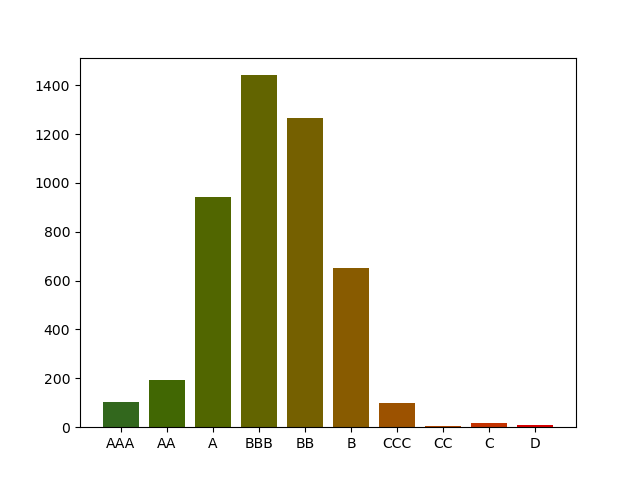
\includegraphics[width=0.95\hsize]{../Output/All Data EDA/Tabular EDA/Distribution of Rating Issuances_no_title.png}
        \end{subfigure}
        %\hfill
        \begin{subfigure}[h]{0.4925\textwidth}
            \centering
            \subcaption{Change Between Fixed Quarter Dates}
            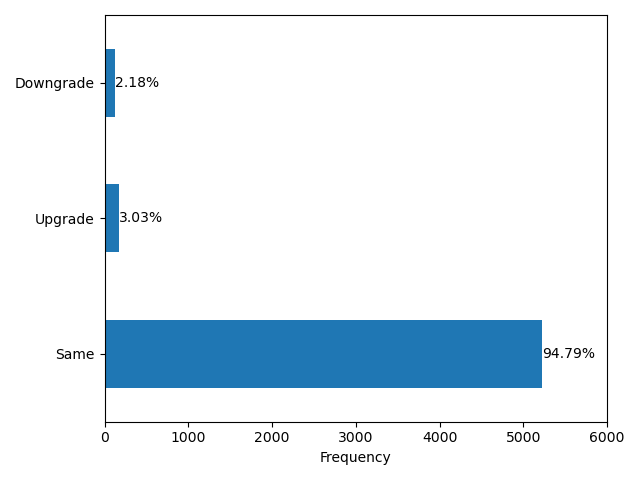
\includegraphics[width=0.95\hsize]{../Output/All Data EDA/Tabular EDA/Change_Short_no_title.png}
        \end{subfigure}
        \hfill
        \label{fig:credit-ratings}
    \end{figure*}

    \subsection*{Earnings Calls}

    Our earnings call data comes from the Financial Modelling Prep API \citep{financial_modeling_prep_financial_2024}, a trusted source widely used in industry. We remove all calls that happened more than 250 days prior and after the year and quarter they are supposed to discuss the results from. Including both prepared remarks and analyst Q and A sessions, the overall average call length in our final data stands at \avgCallLength \space words.

    \subsection*{Financial Statements}

    Our financial statement variables are also retrieved using the Financial Modelling Prep API. We make use of items from company balance sheets, cash flow statements, and income statements, as well as company market capitalization. To prepare the data, we limit our observations to items reported in USD, check for and correct items off by a factor of 1,000 as a result of parsing (if last few digits are 000.00 and the item is above or below 2.5\% and 97.5\% quantile, divide by 1,000), and check some accounting identities in \cite{das_credit_2023}, setting failing variables to missing. We also discard observations where statement filing dates do not agree between the three types of statements, where the filing date falls outside of the fixed quarter matched on via earnings call date, and where the filing date is more than 45 days after the earnings call date.

    \begin{figure*}
        \caption{Altman Z-Score}
        \begin{subfigure}[h]{0.4925\textwidth}
            \centering
            \subcaption{Distribution}
            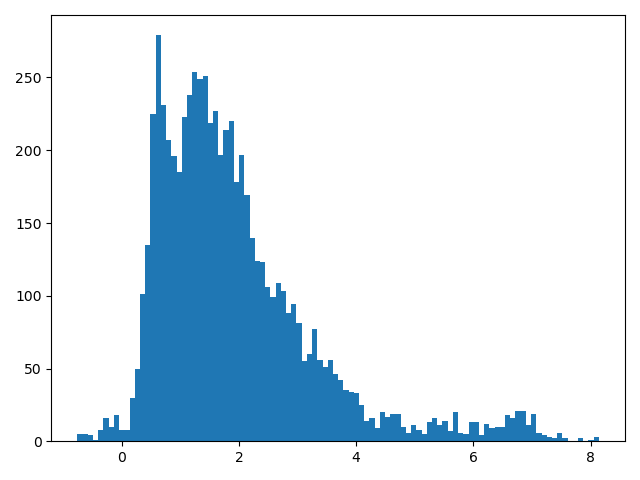
\includegraphics[width=0.95\hsize]{../Output/All Data EDA/Tabular EDA/altman_z_score_all_data_no_title.png}
        \end{subfigure}
        %\hfill
        \begin{subfigure}[h]{0.4925\textwidth}
            \centering
            \subcaption{Average by Rating}
            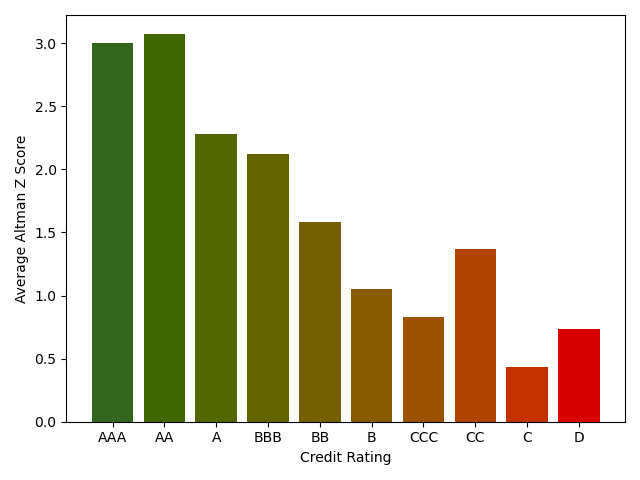
\includegraphics[width=0.95\hsize]{../Output/All Data EDA/Tabular EDA/mean_altman_Z_by_credit_rating_no_title.png}
        \end{subfigure}
        \hfill
        \label{fig:altman-z-score}
    \end{figure*}

    In some of our models, we make use of Altman's Z-score, a traditional measure of bankruptcy risk that accounts for company earnings, equity, and assets and liabilities \citep{altman_financial_1968} (for details on the construction of the score, see Appendix section \ref{sec:altman-z-score}). Figure \ref{fig:altman-z-score} shows the distribution of adjusted Z-scores in our dataset. Traditionally, values above 3.0 have been considered safe, while those below 1.8 are considered to have a high chance of bankruptcy. The average scores for each rating in our data seem to align well with this interpretation, with high scores being associated with higher ratings in a linear manner. Aside from a few quirks on the lower end of the rating spectrum (where not many companies and ratings are available), Z-Score is likely to be highly useful as a predictor.
      
    \subsection*{Sector}

    The GCIS industry classification standard divides companies into 11 major industry sectors (there are finer groupings as well, but this data was not easily obtainable for our project) \citep{s_and_p_gics_2024}. It is widely used in the financial community, and was developed in part by S and P, the same company responsible for our credit ratings. We obtained classifications from Kaggle in CSV format and supplemented them with manual lookup \citep{kozlov_us_2022}. Figure \ref{fig:firms-by-sector} shows the unfortunate sectoral imbalance present in our data, with a large share of firms in consumer, industrial, and technology sectors, relative to very few in the distinctly different financials and real estate sectors.

    \begin{figure*}
        \caption{Sector}
        \begin{subfigure}[h]{0.4925\textwidth}
            \centering
            \subcaption{Firms by Sector}
            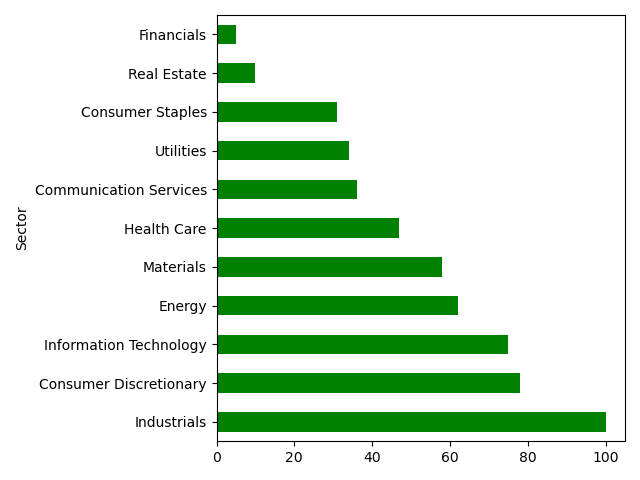
\includegraphics[width=0.95\hsize]{../Output/All Data EDA/Tabular EDA/all_data_fixed_quarter_dates_firms_by_sector_no_title.png}
        \end{subfigure}
        %\hfill
        \begin{subfigure}[h]{0.4925\textwidth}
            \centering
            \subcaption{Average Rating by Sector}
            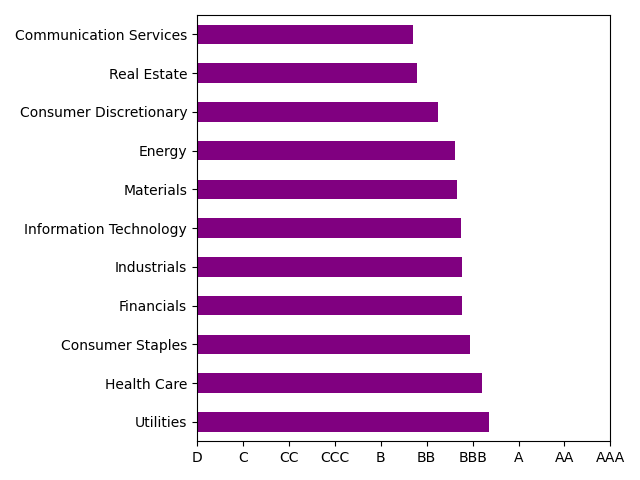
\includegraphics[width=0.95\hsize]{../Output/All Data EDA/Tabular EDA/all_data_fixed_quarter_dates_average_credit_rating_by_sector_no_title.png}
        \end{subfigure}
        \hfill
        \label{fig:firms-by-sector}
    \end{figure*}

    \subsection*{Quality Control}

    Our data preparation was subject to rigorous quality control standards. We extensively code reviewed all data cleaning code. Our exploratory analyses identified data quality issues such as extreme values in financial statement variables, which we handled by winsorizing, and date gaps between quarters, earnings calls, and financial statements, which we dropped in the case of aggregiously mismatched observations.

    \section*{NLP Features}

    Our NLP features capture the sentiment of calls, the transparency of discussion, and the level of analyst engagement.

    \begin{itemize}
        \item Net Positivity Score - In line with \cite{kantos_comparative_2022}, we use the Harvard IV-4 Psychosocial Dictionary \cite{noauthor_inquirer_nodate} to count positive and negative words and compute
        \begin{equation*}
            \text{Net Positivity Score} = log_{10}\frac{\text{Count Positive} + 1}{\text{Count Negative} + 1}
        \end{equation*}
        \item Tone - Following \cite{price_earnings_2012}, we use the Harvard dictionary to count words falling in various categories. Then we construct tone using the first principal component of the matrix with each call as a row and each column as one of the following:
        \begin{equation*}
            \frac{\text{Positive}}{\text{Negative}}, \frac{\text{Active}}{\text{Passive}}, \frac{\text{Strong}}{\text{Weak}}, \frac{\text{Overstated}}{\text{Understated}}
        \end{equation*}
        \item Numeric Transparency - ratio of numbers to words in the word-tokenized call
        \item Readability - We construct the Gunning-Fog readability score \citep{gunning_technique_1952} as 
        \begin{equation*}
            0.4 \times (\frac{\text{Words}}{\text{Sentences}} + 100 \times \frac{\text{3+ Syllable Words}}{\text{Words}})
        \end{equation*}
        \item Number of Questions - count of question marks
    \end{itemize}

    We also add the word count of each call, as this appears to be highly predictive. The distribution of each NLP feature by rating is shown in Figure XXX below.

    INSERT FIGURE

    We are working on preparing FinBERT\footnote{BERT is a pretrained transformer-based language model that encodes text into embedding vectors using surrounding context. FinBERT is a version of BERT finetuned for tasks in the financial domain (language model embedding performance can vary greatly by domain).} \citep{araci_finbert_2019} embeddings and have created Doc2Vec\footnote{This method involves constructing representations of each call based on the bag-of-words and skipgram tasks - a neural network is trained to either a word or a word's context while accounting for a vector identifying the document.} \citep{le_distributed_2014} embeddings to represent sentences and calls. These may be used to improve estimations of sentiment or a direct input to our classifier.

    \section*{Modelling}

    Our overall model architecture is of the form

    \begin{equation*}
        \text{Predicted Credit Rating} = f(\text{Previous Rating}, \text{Metadata}, \text{Financial Variables}, \text{Sector}, \text{NLP Features})
    \end{equation*}

    where Metadata includes relevant date variables from the data sources and the identity of the company and the other variables are as described above.

    \subsection*{Logistic Regression}

    \begin{table*}[h!]
        \centering
        \caption{Model Comparison}
        \footnotesize
\begin{tabular}{cccccc}
\toprule
Model/Baseline & Accuracy & Weighted Average Precision & Weighted Average Recall & F1 Score & Share $\le$ 1 Rating From Actual \\
\midrule
Rating Model 1 & 0.36 & 0.30 & 0.36 & 0.26 & 0.82 \\
Rating Model 2 & 0.51 & 0.49 & 0.51 & 0.46 & 0.89 \\
Rating Model 3 & 0.95 & 0.95 & 0.95 & 0.95 & 0.99 \\
Rating Model 4 & 0.95 & 0.95 & 0.95 & 0.95 & 0.99 \\
Majority Baseline & 0.32 &  &  &  &  \\
\bottomrule
\end{tabular}

\normalsize
        \label{tab:model-comparison}
    \end{table*}

    Table \ref{tab:model-comparison} shows prediction statistics for logistic regression models aiming to predict ratings (for predicting changes in rating, see Appendix Section \ref{sec:change-prediction}). Rating Model 1 includes only Altman's Z-Score as a predictor - its overall accuracy is not much better than the majority baseline, though predictions are generally close to true ratings. Rating Model 2 adds a full suite of financial statement variables (for a list, see items marked as Variable Type `Financial Statements' and `Market Capitalization' in Table \ref{tab:numeric_summary_statistics}) and leads to improvements across the board. Rating Model 3 adds industry sector and the previous rating as predictors, and achieves a very high level of accuracy which we are not currently able to improve upon by adding the NLP features in Rating Model 4.

    \begin{table*}[h!]
        \centering
        \caption{Classification Report - Most Complex Model}
        \small
\begin{tabular}{x{0.75cm}|x{0.75cm}|x{0.75cm}|x{0.75cm}|x{0.75cm}}
\toprule
Rating & Precision & Recall & F1-Score & Support \\
\midrule
AAA & 0.80 & 0.84 & 0.82 & 19 \\
AA & 0.86 & 0.88 & 0.87 & 43 \\
A & 0.93 & 0.92 & 0.92 & 219 \\
BBB & 0.96 & 0.97 & 0.97 & 356 \\
BB & 0.98 & 0.98 & 0.98 & 313 \\
B & 0.97 & 0.95 & 0.96 & 144 \\
CCC & 0.93 & 0.93 & 0.93 & 27 \\
CC & 0.50 & 1.00 & 0.67 & 1 \\
C & 1.00 & 0.67 & 0.80 & 3 \\
D & 1.00 & 1.00 & 1.00 & 2 \\
\bottomrule
\end{tabular}

\normalsize
        \label{tab:most-complex-classification-report}
    \end{table*}

    Table \ref{tab:most-complex-classification-report} generally shows that our most complex model (Rating Model 4) generally performs well across all classes. This is in large part due to our use of balanced class weighting to handle rare classes. We performed grid search 5-fold cross validation to arrive at these balanced weights. We also found via grid search that an Elastic Net penalty (which collapses to entirely a LASSO penalty) with a slight amount of regularization (C) effectively handles the large number of variables present in our data (for details, see Appendix Section \ref{sec:most-complex-model-additional-details}).

    \begin{table*}[h!]
        \centering
        \caption{Permutation Importance - Most Complex Model}
        \footnotesize
\begin{tabular}{ccc}
\toprule
Feature & Mean & Standard Deviation \\
\midrule
Rating on Previous Fixed Quarter Date BBB & 0.281622 & 0.010257 \\
Rating on Previous Fixed Quarter Date BB & 0.230148 & 0.009061 \\
Rating on Previous Fixed Quarter Date A & 0.107111 & 0.005848 \\
Rating on Previous Fixed Quarter Date B & 0.079304 & 0.004862 \\
Rating on Previous Fixed Quarter Date AA & 0.013898 & 0.002093 \\
Rating on Previous Fixed Quarter Date CCC & 0.012949 & 0.001282 \\
Total Non-Current Liabilities & 0.000867 & 0.000612 \\
Total Stockholders' Equity & 0.000809 & 0.000366 \\
Research and Development Expenses & 0.000789 & 0.000284 \\
Net Receivables & 0.000779 & 0.000314 \\
Gunning-Fog Score & 0.000764 & 0.000307 \\
Dividends Paid & 0.000663 & 0.000504 \\
Other Current Liabilities & 0.000659 & 0.000388 \\
Debt Repayment & 0.000631 & 0.000402 \\
Numeric Transparency & 0.000543 & 0.000469 \\
\bottomrule
\end{tabular}

\normalsize
        \label{tab:most-complex-permutation-importance}
    \end{table*}

    \section*{Conclusion and Next Steps}

    We have seen above that textual and NLP features are contributing to our predictions...

    One major next step is continuing to improve the construction of our NLP features and methods. Much more work could be done to improve the construction of our sentiment scores and analysis - seeking out better pretrained models for earnings call sentiment, or improving the methods through which embedding representations are converted to sentiment. Some members of the group have also been working on a separate class project involving annotating earnings calls with topics discussed. This work could be integrated into our project to provide additional features for our models - we could identity topics and then connect them to credit ratings. Finally, we could try building an end-to-end transformer classifier that takes in earnings calls and outputs credit ratings (perhaps finetuning and adding a classifier on top of the longformer \citep{beltagy_longformer_2020} transformer encoder model\footnote{Longformer or other techniques are ideal for document, rather than word or sentence embedding creation}).

    We've also begun using the AutoML library Autogluon to explore a wider variety of classifiers. Autogluon runs a wide variety of state-of-the-art prediction algorithms and performs hyperparameter tuning. The results, shown in Table \ref{tab:autogluon-leaderboard} for all allowed predictors in our dataset (metadata about call and statement dates, the rating on the previous fixed quarter date, all the financial statement variables, all the constructed NLP features, and sector) can provide a good starting point for our further modelling choices.

    \begin{table*}[h!]
        \centering
        \caption{Autogluon Leaderboard}
        \begin{tabular}{lr}
\toprule
Model & Test Accuracy \\
\midrule
XGBoost & 0.953860 \\
LightGBM & 0.952972 \\
LightGBMXT & 0.952972 \\
WeightedEnsembleL2 & 0.952972 \\
CatBoost & 0.952085 \\
NeuralNetTorch & 0.950311 \\
LightGBMLarge & 0.943212 \\
ExtraTreesGini & 0.939663 \\
ExtraTreesEntr & 0.938776 \\
RandomForestGini & 0.937888 \\
NeuralNetFastAI & 0.935226 \\
RandomForestEntr & 0.934339 \\
KNeighborsDist & 0.874002 \\
KNeighborsUnif & 0.848270 \\
\bottomrule
\end{tabular}

        \label{tab:autogluon-leaderboard}
    \end{table*}

    Tree-based bagging and boosting methods (boosting in particular) seem to perform extraordinarily well on our modelling task (ExtraTrees is a somewhat simplified variant of random forest; GBM stands for Gradient Boosting Machine). Each of the trained Autogluon models also comes with a set of optimized hyperparameters - after selecting a model, we will further tune these hyperparameters to improve performance. The library also provides feature importance measures, computed by permuting each feature and measuring the drop in accuracy. Though these tests are not of high quality (and many results are not reported or are not significant), they confirm that previous ratings, earnings call word counts and tone variables, a few financial variables, and several date metadate variables are all very important.

    CATEGORICAL PREVIOUS RATING IS THE MOST IMPORTANT PREDICTOR

    Another area of interest for us is continuing to pursue the approach in \cite{das_credit_2023}, which uses graph neural networks to model the relationships between companies in combination with tabular financial data and NLP features. Prerequisite to this approach is the construction of an undirected graph showing linkages between companies based on the earnings call data. We've pursued begun work on this step from two angles. First, following the original paper, Doc2Vec embeddings representing calls can be averaged for each company. A graph can then be constructed with connecting edges added for cases when the vectors for each company have cosine similarity above a certain threshhold. As a second approach, which also opens more opportunities for exploration even without a neural network, we have used transformer-based Named Entity Recognition to identify mentions of any company in each earnings call. On average, each earnings call has \avgCompanyMentions \space company mentions - Figure \ref{fig:company-mentions} shows the distribution.

    \begin{figure}[h!]
		\centering
        \caption{Company Mentions}
        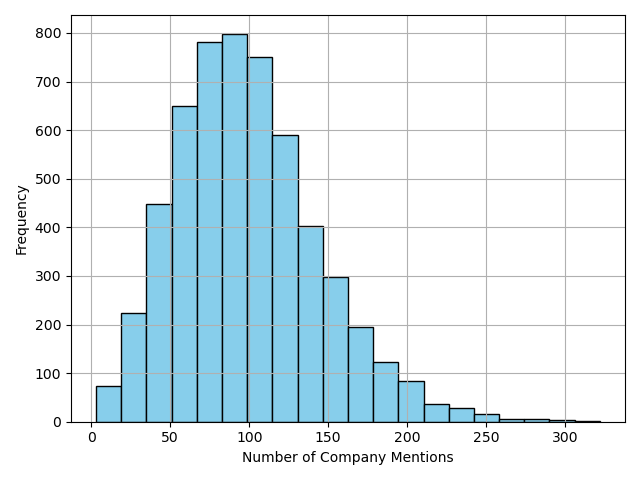
\includegraphics[width=0.4925\textwidth,keepaspectratio=true]{../Output/All Data EDA/NLP EDA - NER on Company Names/Company Mentions Distribution No Title.png}
        \label{fig:company-mentions}
	\end{figure}

    Though the vast majority of these mentions are likely to be of the company whose call is being discussed, a casual glance at the data does suggest there are a fair number of mentions of partners, suppliers, and competitors within some calls. Our next step involves the use of entity resolution algorithms (trigram matching, supervised learning) to link these mentions to firm tickers in order to construct a graph of relationships.
    
    \section*{Acknowledgements}

    Special thanks to the UC Berkeley Stats Department Statistical Computing Facility (SCF). Other acknowledgements: Libor Pospisil, Robert Thompson. GitHub Co-Pilot was used for python code generation (mostly for plotting and table creation/parsing).

    \clearpage
    \newpage

    \bibliographystyle{aea}
    \bibliography{Stat-222-Capstone}

    \clearpage
    \newpage

    \appendix

    % Reset and change numbering for figures and tables
    \counterwithin{figure}{section}
    \counterwithin{table}{section}

    \section{Appendix}

    \subsection{Summary Statistics for Numeric Variables}

    Table \ref{tab:numeric_summary_statistics} shows summary statistics for all numeric variables in our dataset. Important numeric and categorical variables are explained in the main text. We also have numerous date variables, which we may use in future predictions.

    \begin{tabular}{lcccccc}
 & Mean & Minimum & Median & Maximum & Standard Deviation & Variable Type \\
Variable Name &  &  &  &  &  &  \\
Altman's Z Score & 1.88 & -0.91 & 1.58 & 7.56 & 1.30 & Altman's Z Score \\
Accounts Payable (Balance Sheet) & 928,879,944.12 & -237,651,171.00 & 338,150,000.00 & 11,433,000,000.00 & 1,529,128,185.80 & Financial Statements \\
Accounts Payable (Cash Flow Statement) & 4,706,860.62 & -321,769,000.00 & 0.00 & 1,789,652,000.00 & 80,197,009.20 & Financial Statements \\
Accounts Receivables & -10,753,743.96 & -542,000,000.00 & 0.00 & 321,200,000.00 & 90,085,627.31 & Financial Statements \\
Accumulated Other Comprehensive Income (Loss) & -381,975,004.44 & -5,242,000,000.00 & -74,116,000.00 & 431,595,000.00 & 840,987,604.56 & Financial Statements \\
Capital Expenditure & -193,647,213.17 & -1,867,000,000.00 & -59,608,703.91 & 412,700.00 & 314,135,930.83 & Financial Statements \\
Capital Lease Obligations & 28,065,070.59 & 0.00 & 0.00 & 9,056,234,000.00 & 244,927,479.06 & Financial Statements \\
Cash and Cash Equivalents & 852,349,405.25 & 0.00 & 303,118,000.00 & 9,204,000,000.00 & 1,382,415,295.39 & Financial Statements \\
Cash and Short Term Investments & 1,029,007,733.36 & 0.00 & 328,148,000.00 & 15,601,000,000.00 & 1,875,370,693.02 & Financial Statements \\
Cash at Beginning of Period & 857,491,604.07 & -2,556,000.00 & 306,627,000.00 & 9,610,000,000.00 & 1,410,191,719.21 & Financial Statements \\
Cash at End of Period & 866,528,388.67 & -154,400.00 & 307,677,500.00 & 9,743,000,000.00 & 1,425,442,968.51 & Financial Statements \\
Change in Working Capital & -16,292,925.52 & -870,000,000.00 & -1,898,000.00 & 756,000,000.00 & 180,310,959.28 & Financial Statements \\
Common Stock & 332,954,612.87 & -539,800.00 & 3,900,000.00 & 9,817,134,000.00 & 917,174,360.11 & Financial Statements \\
Common Stock Issued & 45,711,557.87 & -3,572,000.00 & 26,500.00 & 906,500,000.00 & 125,660,488.08 & Financial Statements \\
Common Stock Repurchased & -74,290,519.19 & -1,135,000,000.00 & -400,000.00 & 545,656,614.52 & 181,665,328.82 & Financial Statements \\
Cost and Expenses & 2,329,299,450.91 & -2,495,000.00 & 1,109,876,000.00 & 22,496,000,000.00 & 3,409,414,855.37 & Financial Statements \\
Cost of Revenue & 1,630,285,860.24 & -3,094,000.00 & 773,300,000.00 & 16,948,000,000.00 & 2,425,958,117.19 & Financial Statements \\
Debt Repayment & -260,678,959.19 & -3,001,000,000.00 & -35,000,000.00 & 200.00 & 490,067,002.19 & Financial Statements \\
Deferred Income Tax & 5,769,703.18 & -253,000,000.00 & 50,500.00 & 1,850,454,000.00 & 60,203,360.61 & Financial Statements \\
Deferred Revenue & 301,721,276.89 & -116,912,000.00 & 47,100,000.00 & 4,918,100,000.00 & 643,876,051.90 & Financial Statements \\
Depreciation and Amortization (Cash Flow Statement) & 145,689,205.06 & -304,000.00 & 53,427,500.00 & 1,529,000,000.00 & 218,965,861.00 & Financial Statements \\
Depreciation and Amortization (Income Statement) & 142,779,168.92 & -1,550,000.00 & 53,593,000.00 & 1,371,000,000.00 & 210,651,321.79 & Financial Statements \\
Diluted EPS & 0.49 & -156.36 & 0.51 & 49.73 & 3.53 & Financial Statements \\
Dividends Paid & -93,842,514.12 & -1,233,000,000.00 & -21,783,000.00 & 0.00 & 186,830,876.64 & Financial Statements \\
EBITDA & 447,620,359.75 & -66,200,000.00 & 191,346,000.00 & 4,410,000,000.00 & 657,882,497.84 & Financial Statements \\
EBITDA Ratio & 0.20 & -5.77 & 0.18 & 2.16 & 0.23 & Financial Statements \\
EPS & 0.50 & -156.36 & 0.52 & 53.75 & 3.56 & Financial Statements \\
Effect of Foreign Exchange Changes on Cash & -1,647,078.82 & -65,000,000.00 & 0.00 & 52,000,000.00 & 10,955,813.05 & Financial Statements \\
Free Cash Flow & 152,488,089.91 & -541,000,000.00 & 50,350,500.00 & 2,683,000,000.00 & 386,075,408.86 & Financial Statements \\
General and Administrative Expenses & 142,016,375.14 & -2,117,000.00 & 30,257,000.00 & 2,007,000,000.00 & 288,668,731.35 & Financial Statements \\
Goodwill & 1,971,783,101.42 & -202,702,100.00 & 626,536,500.00 & 23,389,000,000.00 & 3,541,028,978.34 & Financial Statements \\
Goodwill and Intangible Assets & 3,143,944,231.55 & -1,618,944,000.00 & 962,312,000.00 & 37,123,000,000.00 & 5,784,596,899.63 & Financial Statements \\
Gross Profit & 872,368,464.63 & -7,195,000.00 & 373,018,500.00 & 9,223,000,000.00 & 1,421,025,818.62 & Financial Statements \\
Gross Profit Ratio & 0.37 & -5.65 & 0.34 & 2.19 & 0.27 & Financial Statements \\
Income Before Tax & 249,496,947.58 & -353,153,000.00 & 89,895,500.00 & 2,951,000,000.00 & 434,495,406.26 & Financial Statements \\
Income Before Tax Ratio & 0.07 & -9.38 & 0.09 & 1.27 & 0.37 & Financial Statements \\
Income Tax Expense & 68,390,107.98 & -119,131,000.00 & 21,775,500.00 & 736,000,000.00 & 121,599,241.07 & Financial Statements \\
Intangible Assets & 869,968,811.22 & -421,000.00 & 173,358,000.00 & 14,110,100,000.00 & 1,855,409,062.61 & Financial Statements \\
Interest Expense & 49,203,706.71 & -16,400,000.00 & 23,385,000.00 & 386,000,000.00 & 65,029,625.22 & Financial Statements \\
Interest Income & 2,335,687.82 & -32,293.00 & 0.00 & 69,000,000.00 & 6,967,205.85 & Financial Statements \\
Inventory (Balance Sheet) & 958,995,636.94 & -19,626,000.00 & 414,950,000.00 & 8,328,000,000.00 & 1,433,396,913.56 & Financial Statements \\
Inventory (Cash Flow Statement) & -10,636,842.51 & -420,000,000.00 & 0.00 & 289,000,000.00 & 70,202,756.90 & Financial Statements \\
Investments in Property, Plants, and Equipment & -194,860,014.81 & -1,921,864,000.00 & -59,719,000.00 & 412,700.00 & 317,067,486.90 & Financial Statements \\
Long-Term Debt & 4,342,642,310.38 & 0.00 & 1,843,812,000.00 & 31,228,000,000.00 & 5,794,340,264.76 & Financial Statements \\
Long-Term Investments & 521,054,256.46 & -490,677,000.00 & 11,203,500.00 & 10,981,000,000.00 & 1,427,052,488.42 & Financial Statements \\
Minority Interest & 96,515,825.94 & -286,000.00 & 1,784,000.00 & 2,316,406,000.00 & 283,036,455.78 & Financial Statements \\
Net Acquisitions & -31,252,849.61 & -805,960,000.00 & 0.00 & 249,000,000.00 & 113,700,319.45 & Financial Statements \\
Net Cash Provided by Operating Activities & 353,695,946.55 & -175,500,000.00 & 142,068,000.00 & 3,870,000,000.00 & 559,577,854.70 & Financial Statements \\
Net Cash Used for Investing Activities & -252,301,738.93 & -2,840,033,000.00 & -69,018,000.00 & 325,900,000.00 & 447,680,994.35 & Financial Statements \\
Net Cash Used or Provided by Financing Activities & -113,094,742.90 & -2,444,000,000.00 & -28,913,000.00 & 1,094,000,000.00 & 398,976,123.98 & Financial Statements \\
Net Change in Cash & 6,986,471.31 & -1,161,000,000.00 & 326,500.00 & 1,401,000,000.00 & 262,805,651.94 & Financial Statements \\
Net Debt & 3,807,913,408.87 & -1,044,500,000.00 & 1,567,100,000.00 & 30,761,000,000.00 & 5,555,751,832.58 & Financial Statements \\
Net Income (Cash Flow Statement) & 186,107,161.79 & -327,000,000.00 & 64,393,500.00 & 2,402,000,000.00 & 338,084,813.74 & Financial Statements \\
Net Income (Income Statement) & 183,234,857.90 & -329,864,000.00 & 64,300,000.00 & 2,340,000,000.00 & 335,149,633.65 & Financial Statements \\
Net Income Ratio & 0.05 & -8.88 & 0.07 & 2.72 & 0.31 & Financial Statements \\
Net Property Plant Equipment & 5,007,874,719.10 & 0.00 & 1,389,082,500.00 & 44,441,000,000.00 & 8,045,435,934.42 & Financial Statements \\
Net Receivables & 1,259,577,298.60 & -4,199,600.00 & 539,100,000.00 & 12,146,000,000.00 & 1,814,088,013.82 & Financial Statements \\
Non-Current Deferred Revenue & 250,512,754.02 & -500,933,000.00 & 0.00 & 5,778,000,000.00 & 727,888,527.14 & Financial Statements \\
Non-Current Deferred Tax Liabilities & 698,746,738.38 & -3,818,507.00 & 133,077,500.00 & 8,306,000,000.00 & 1,425,671,155.54 & Financial Statements \\
Operating Cash Flow & 353,695,946.55 & -175,500,000.00 & 142,068,000.00 & 3,870,000,000.00 & 559,577,854.70 & Financial Statements \\
Operating Expenses & 547,725,941.27 & -13,530,000.00 & 211,937,500.00 & 6,252,000,000.00 & 959,936,714.19 & Financial Statements \\
Operating Income & 298,743,632.43 & -208,377,000.00 & 119,850,000.00 & 3,294,000,000.00 & 476,982,715.49 & Financial Statements \\
Operating Income Ratio & 0.10 & -9.71 & 0.12 & 1.14 & 0.33 & Financial Statements \\
Other Assets & 8,191.33 & -19,834,700.00 & 0.00 & 8,948,000.00 & 468,348.06 & Financial Statements \\
Other Current Assets & 380,708,173.61 & -49,000.00 & 113,056,500.00 & 4,968,950,000.00 & 690,346,469.76 & Financial Statements \\
Other Current Liabilities & 990,758,356.70 & -48,317,000.00 & 322,670,500.00 & 12,137,000,000.00 & 1,870,004,710.84 & Financial Statements \\
Other Expenses & 49,916,440.59 & -64,000,000.00 & 608,500.00 & 16,189,674,590.00 & 363,247,062.24 & Financial Statements \\
Other Financing Activities & 221,463,311.27 & -975,168,999.00 & 8,000,000.00 & 3,297,501,000.00 & 524,943,949.61 & Financial Statements \\
Other Investing Activities & 4,791,113.98 & -448,000,000.00 & 123,500.00 & 3,060,433,659.00 & 97,646,984.87 & Financial Statements \\
Other Liabilities & 111,303.72 & -267,212.00 & 0.00 & 51,076,000.00 & 2,208,107.68 & Financial Statements \\
Other Non-Cash Items & 14,733,647.77 & -1,848,719,007.00 & 1,562,000.00 & 699,000,000.00 & 105,972,613.46 & Financial Statements \\
Other Non-Current Assets & 526,230,472.94 & -75,012,534,818.00 & 154,478,500.00 & 8,037,000,000.00 & 1,892,020,258.31 & Financial Statements \\
Other Non-Current Liabilities & 973,607,594.44 & -286,041,895.00 & 326,195,000.00 & 11,890,564,000.00 & 1,729,729,702.42 & Financial Statements \\
Other Total Stockholders' Equity & 1,058,480,401.28 & -12,393,000,000.00 & 387,440,500.00 & 34,030,400,000.00 & 3,676,996,160.82 & Financial Statements \\
Other Working Capital & 20,095,755.18 & -1,788,851,160.00 & 0.00 & 40,341,689,407.00 & 784,774,785.47 & Financial Statements \\
Preferred Stock & 8,957,412.19 & 0.00 & 0.00 & 401,500,000.00 & 41,741,915.35 & Financial Statements \\
Purchases of Investments & -99,111,435.92 & -11,997,654,000.00 & 0.00 & 81,823,000.00 & 344,843,591.76 & Financial Statements \\
Research and Development Expenses & 24,546,760.47 & -214,000.00 & 0.00 & 893,000,000.00 & 90,083,795.75 & Financial Statements \\
Retained Earnings & 3,629,692,655.97 & -4,839,000,000.00 & 1,274,232,500.00 & 37,899,000,000.00 & 6,497,897,135.46 & Financial Statements \\
Revenue & 2,752,115,994.55 & -4,273,000.00 & 1,283,674,000.00 & 25,420,000,000.00 & 4,046,436,838.80 & Financial Statements \\
Sales and Maturities of Investments & 92,477,266.23 & -9,409,000.00 & 0.00 & 8,936,406,000.00 & 303,356,990.01 & Financial Statements \\
Selling General and Administrative Expenses & 293,844,085.52 & -2,117,000.00 & 114,052,500.00 & 3,333,000,000.00 & 495,298,108.22 & Financial Statements \\
Selling and Marketing Expenses & 25,337,708.44 & -3,003,000.00 & 0.00 & 876,761,000.00 & 98,783,957.01 & Financial Statements \\
Short Term Investments & 171,674,306.11 & -515,000.00 & 0.00 & 6,178,000,000.00 & 570,578,944.19 & Financial Statements \\
Short-Term Debt & 488,398,947.44 & -655,561.00 & 89,034,500.00 & 5,359,000,000.00 & 919,311,633.83 & Financial Statements \\
Stock-Based Compensation & 14,271,901.15 & -36,000,000.00 & 4,956,500.00 & 254,000,000.00 & 30,389,470.84 & Financial Statements \\
Tax Assets & 374,484,728.56 & -2,310,712,000.00 & 45,781,000.00 & 6,535,000,000.00 & 917,009,577.63 & Financial Statements \\
Tax Payable & 60,320,998.32 & -87,400.00 & 2,916,000.00 & 1,183,200,000.00 & 151,310,152.81 & Financial Statements \\
Total Assets & 16,041,516,101.31 & 123,279.00 & 6,776,797,500.00 & 131,556,000,000.00 & 22,888,760,450.42 & Financial Statements \\
Total Current Assets & 3,956,106,957.32 & 35,587.00 & 1,887,586,000.00 & 41,276,000,000.00 & 5,914,890,504.74 & Financial Statements \\
Total Current Liabilities & 2,841,825,102.84 & 12,178.00 & 1,101,173,000.00 & 29,919,000,000.00 & 4,386,480,010.78 & Financial Statements \\
Total Debt & 4,788,891,751.88 & 2,000.00 & 2,037,148,000.00 & 37,124,000,000.00 & 6,477,270,025.47 & Financial Statements \\
Total Equity & 5,025,612,554.17 & -501,467,000.00 & 2,029,718,000.00 & 49,975,000,000.00 & 7,546,463,280.10 & Financial Statements \\
Total Investments & 762,733,616.78 & -334,673,000.00 & 38,129,000.00 & 19,331,000,000.00 & 2,065,926,624.79 & Financial Statements \\
Total Liabilities & 10,144,020,041.90 & 79,283.00 & 4,287,428,500.00 & 87,293,000,000.00 & 14,121,143,146.21 & Financial Statements \\
Total Liabilities and Stockholders' Equity & 16,005,558,652.32 & 123,279.00 & 6,776,797,500.00 & 131,556,000,000.00 & 22,880,811,656.54 & Financial Statements \\
Total Liabilities and Total Equity & 16,005,558,652.32 & 123,279.00 & 6,776,797,500.00 & 131,556,000,000.00 & 22,880,811,656.54 & Financial Statements \\
Total Non-Current Assets & 11,376,619,839.67 & 49,861.00 & 4,137,290,500.00 & 104,263,000,000.00 & 16,727,793,153.36 & Financial Statements \\
Total Non-Current Liabilities & 6,875,270,635.58 & 53,696.00 & 2,800,400,000.00 & 54,300,000,000.00 & 9,789,172,194.03 & Financial Statements \\
Total Other Income Expenses Net & -12,311,364.49 & -503,976,000.00 & -795,000.00 & 286,000,000.00 & 72,409,332.85 & Financial Statements \\
Total Stockholders' Equity & 4,987,566,971.51 & -526,491,000.00 & 2,028,600,000.00 & 49,269,000,000.00 & 7,466,218,430.87 & Financial Statements \\
Weighted Average Shares Outstanding & 361,410,798.65 & 0.00 & 145,598,222.50 & 13,751,391,147.00 & 752,501,668.54 & Financial Statements \\
Weighted Average Shares Outstanding (Diluted) & 322,626,084.79 & 0.00 & 144,583,000.00 & 13,986,214,405.00 & 577,545,825.69 & Financial Statements \\
Market Capitalization & 20,034,247,568.22 & 106,422.00 & 6,348,776,650.00 & 726,320,349,360.00 & 47,265,667,703.74 & Market Capitalization \\
Days Since Call & 58.21 & 0.00 & 61.00 & 91.00 & 13.30 & Metadata \\
First Principal Component of Tone & -0.01 & -2.64 & -0.20 & 25.35 & 1.34 & NLP Feature \\
Gunning-Fog Score & 12.52 & 8.55 & 12.43 & 19.29 & 1.32 & NLP Feature \\
Number of Questions & 36.24 & 0.00 & 35.00 & 107.00 & 16.29 & NLP Feature \\
Numeric Transparency & 0.12 & 0.01 & 0.12 & 0.40 & 0.05 & NLP Feature \\
Postitivity Score & 0.19 & -0.20 & 0.18 & 0.65 & 0.10 & NLP Feature \\
Readability & 12.52 & 8.55 & 12.43 & 19.29 & 1.32 & NLP Feature \\
Word Count & 8,851.58 & 1,782.00 & 9,077.00 & 22,006.00 & 2,489.13 & NLP Feature \\
Change Since Last Fixed Quarter Date & 0.01 & -2.00 & 0.00 & 2.00 & 0.29 & Predicted - Change \\
\end{tabular}


    \clearpage
    \newpage

    \subsection{Observations by Quarter and Year}

    Figure \ref{fig:obs-by-quarter-year} demonstrates that the data is temporally unbalanced, with many companies entering the dataset in later years, after they first receive an observable credit rating.

    \begin{figure}[h!]
		\centering
        \caption{Observations by Quarter and Year}
        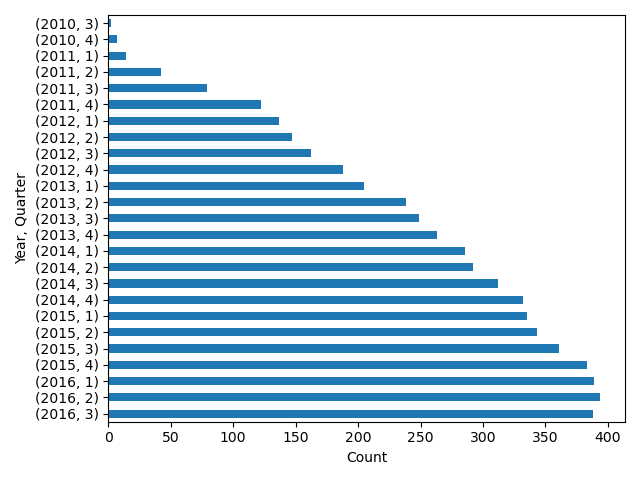
\includegraphics[width=0.6\linewidth,keepaspectratio=true]{../Output/All Data EDA/Tabular EDA/all_data_fixed_quarter_dates_obs_by_year_quarter_no_title.png}
        \label{fig:obs-by-quarter-year}
	\end{figure}

    \clearpage
    \newpage

    \subsection{Altman's Z-Score}

    \label{sec:altman-z-score}

    As in \cite{das_credit_2023}, the components of the Z-score are as follows:

    \begin{itemize}
        \item A: EBIT / Total Assets
        \item B: Net Sales / Total Assets
        \item C: Market Capitalization / Total Liabilities
        \item D: Working Capital / Total Assets
        \item E: Retained Earnings / Total Assets
    \end{itemize}

    We Winsorize extreme values of Ratio A, B, D, and E by setting the top and bottom 2.5\% of values to the 97.5 and 2.5 percentile, respectively. Due to the presence of additional outliers and the sourcing of market capitalization from a different dataset than the rest of the variables, Ratio C is instead Winsorized over the top and bottom 5\% of values. 

    The ratios are combined via the following equation:

    \begin{equation*}
        \text{Z-Score} = 3.3 A + 0.99 B + 0.6 C + 1.2 D + 1.4 E
    \end{equation*}

    \clearpage
    \newpage
    \subsection{Logistic Regression - Most Complex Model - Additional Details}

    \label{sec:most-complex-model-additional-details}

    \begin{table*}[h!]
        \centering
        \caption{Best Hyperparameters - Most Complex Model}
        \small
\begin{tabular}{cccccc}
\toprule
C & Class Weighting Strategy & L1 Ratio & Multi-Class Strategy & Penalty & Solver \\
\midrule
0.100000 & Balanced & 1.000000 & One vs Rest & Elastic Net & SAGA \\
\bottomrule
\end{tabular}

\normalsize
        \label{tab:most-complex-best-params}
    \end{table*}

    \begin{figure}[h!]
		\centering
        \caption{Confusion Matrix - Most Complex Model}
        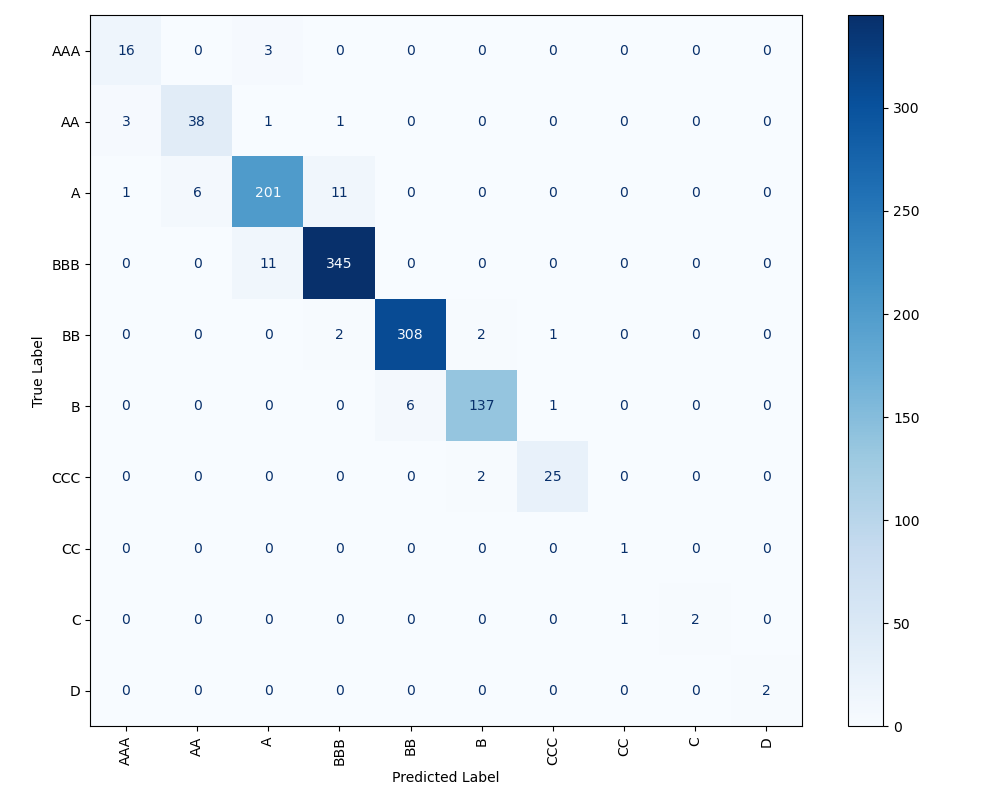
\includegraphics[width=0.6\linewidth,keepaspectratio=true]{../Output/Modelling/Logistic Regression/rating_model_4/rating_model_4_confusion_matrix_no_title.png}
        \label{fig:most-confusion-matrix}
	\end{figure}

    \clearpage
    \newpage

    \subsection{Logistic Regression - Predicting Changes in Rating}

    \label{sec:change-prediction}

    Table \ref{tab:change-prediction} shows that our most complex model (with the same variables as Rating Model 4) is able to predict changes in rating with a high degree of accuracy, and the weighted average statistics are as expected. Figure \ref{fig:change-confusion-matrix} displays the confusion matrix. We fine-tuned our hyperHyperparameters for this model with an accuracy objective, and so grid search was allowed to completely ignores the non-majority classes and not perform balanced class weighting. More work is needed to either force balance weighting or change the grid search objective.

    \begin{table*}[h!]
        \centering
        \caption{Classification Report - Change Prediction}
        \footnotesize
\begin{tabular}{ccccc}
\toprule
Accuracy & Weighted Average Precision & Weighted Average Recall & F1 Score & Majority Baseline \\
\midrule
0.96 & 0.91 & 0.96 & 0.93 & 0.96 \\
\bottomrule
\end{tabular}

\normalsize
        \label{tab:change-prediction}
    \end{table*}

    \begin{figure}[h!]
		\centering
        \caption{Confusion Matrix - Changes in Rating}
        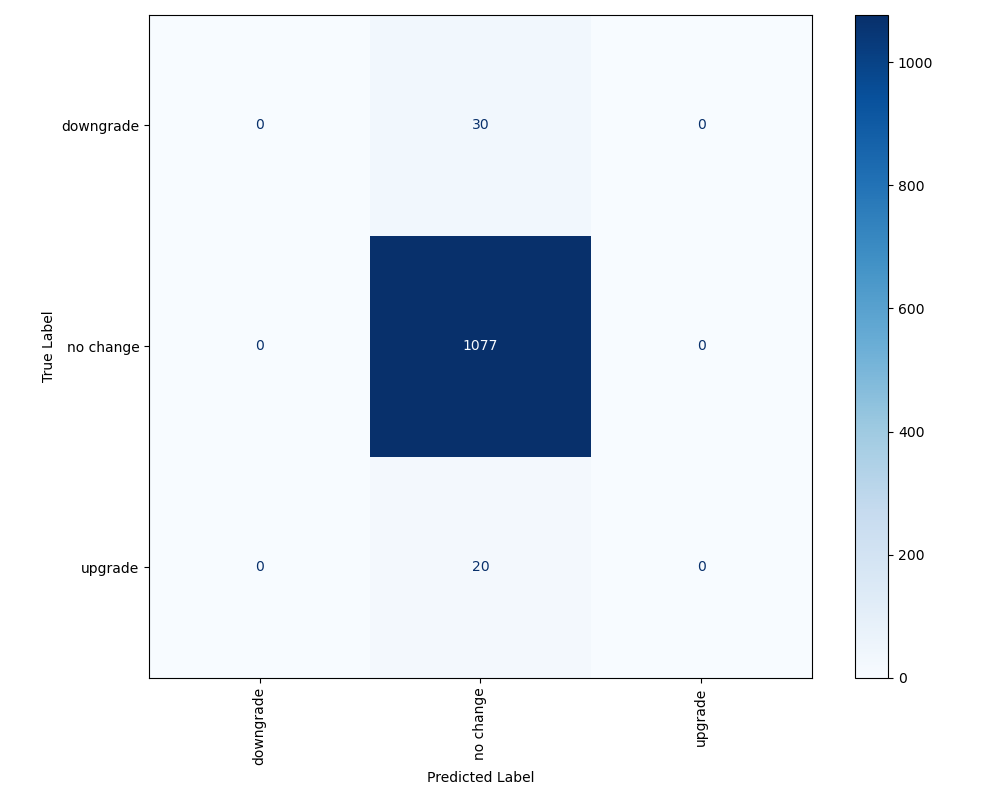
\includegraphics[width=0.6\linewidth,keepaspectratio=true]{../Output/Modelling/Logistic Regression/change_model/change_model_confusion_matrix_no_title.png}
        \label{fig:change-confusion-matrix}
	\end{figure}


\end{document}
